\section{Discussions} \label{sec:discussion}
In this section, we discuss the evolution of low-code and LCSD related discussions with respect to different topics. Then we discuss the implications of our findings. 


% \subsubsection{Results}
\subsection{Evolution of LCSD topics}
% \gias{First, show a graph of overall post relative growth similar to Chatbot paper~\cite{abdellatif2020challenges}. Then show a graph like Fig. 3 from Chatbot paper. Now explain drop in \# posts in that figure in 2020 by disclosing about Google App maker. Finally show the evolution per platform, that chart you showed me. Now discuss the types of challenges developers discussed about Google app maker before and after the discontinuation notice. Compare whether 
% the challenge types and their frequencies differ between app maker and saleforce pre and post Jan 2020.
% Also see if you can explain any other change (e.g., up or down swing of a topic category over time).}

% Google app maker
% January 27, 2020: Existing apps continue to work. Though App Maker is no longer under active development, the service will continue to be maintained.
% April 15, 2020: You will no longer be able to create new App Maker apps. You will still be able to edit and deploy existing apps.
% January 19, 2021: Existing App Maker apps will stop working and you will no longer have access to them.

We measure the growth of our four high-level topic categories over time to better understand the evolution of LCSD. We measure the absolute growth, i.e., the total number of questions in a category over time. Figure ~\ref{fig:trend_questions_per_topic_category} shows that all four of our topic categories are increasing monotonically.
% This trend suggests an increasing number of queries in each category, which also means an increasing trend of development activities under each category. 
This trend indicates that the LCSD approach is gaining more community attention over time, especially after 2016. 
\begin{figure}[t]
\centering
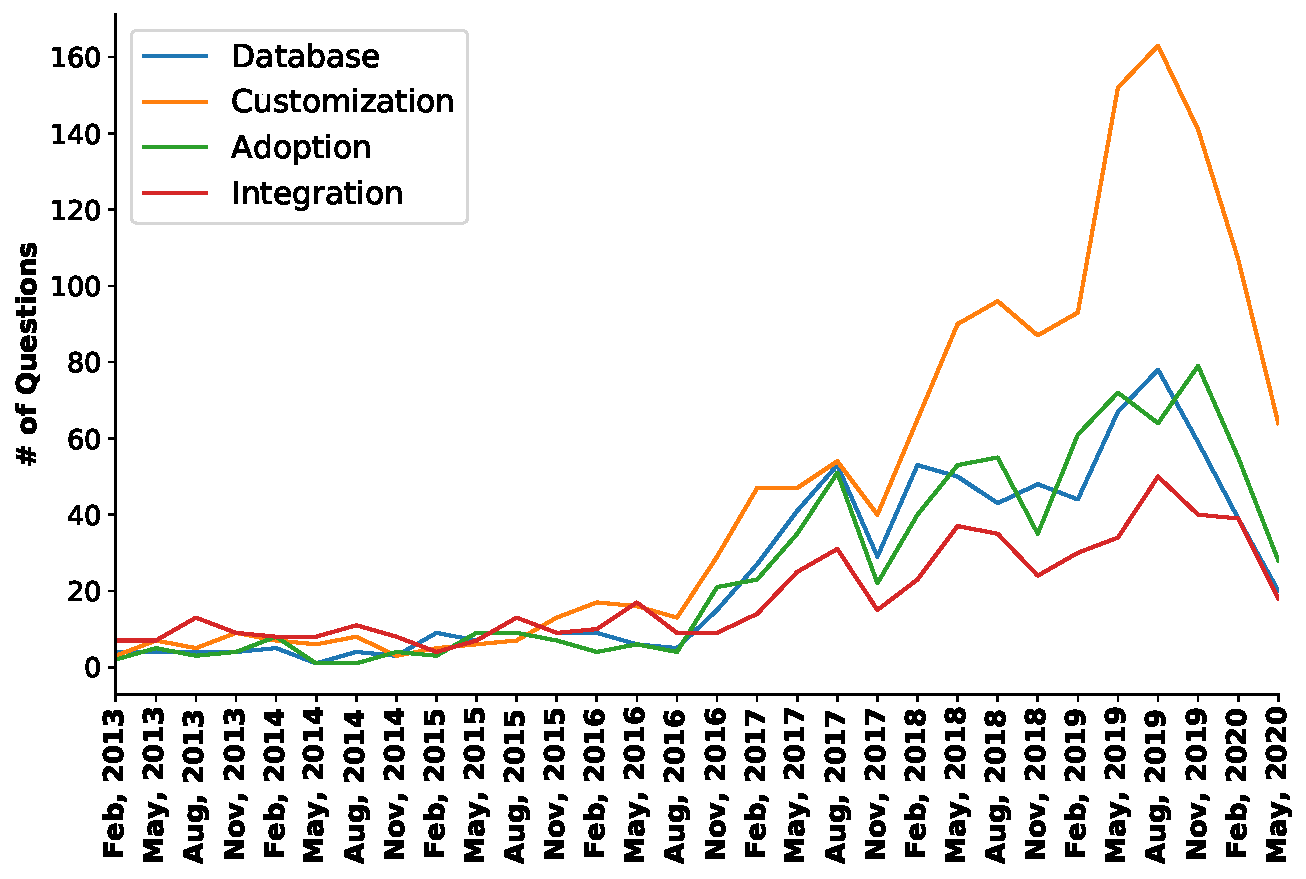
\includegraphics[scale=0.38]{res/Question_per_higher_category_3M.pdf}
% 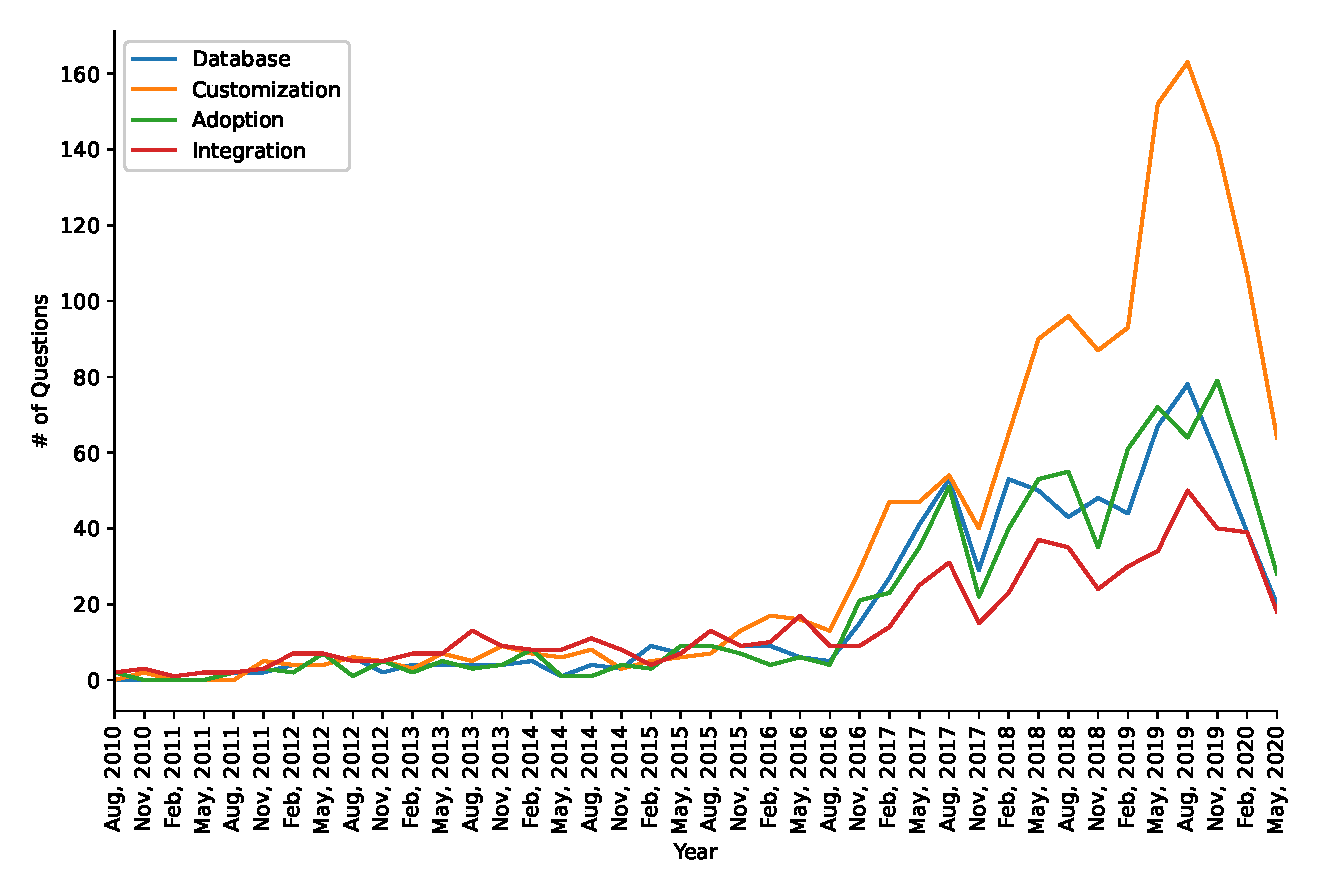
\includegraphics[scale=0.38]{res/Question_per_higher_category.eps}
% 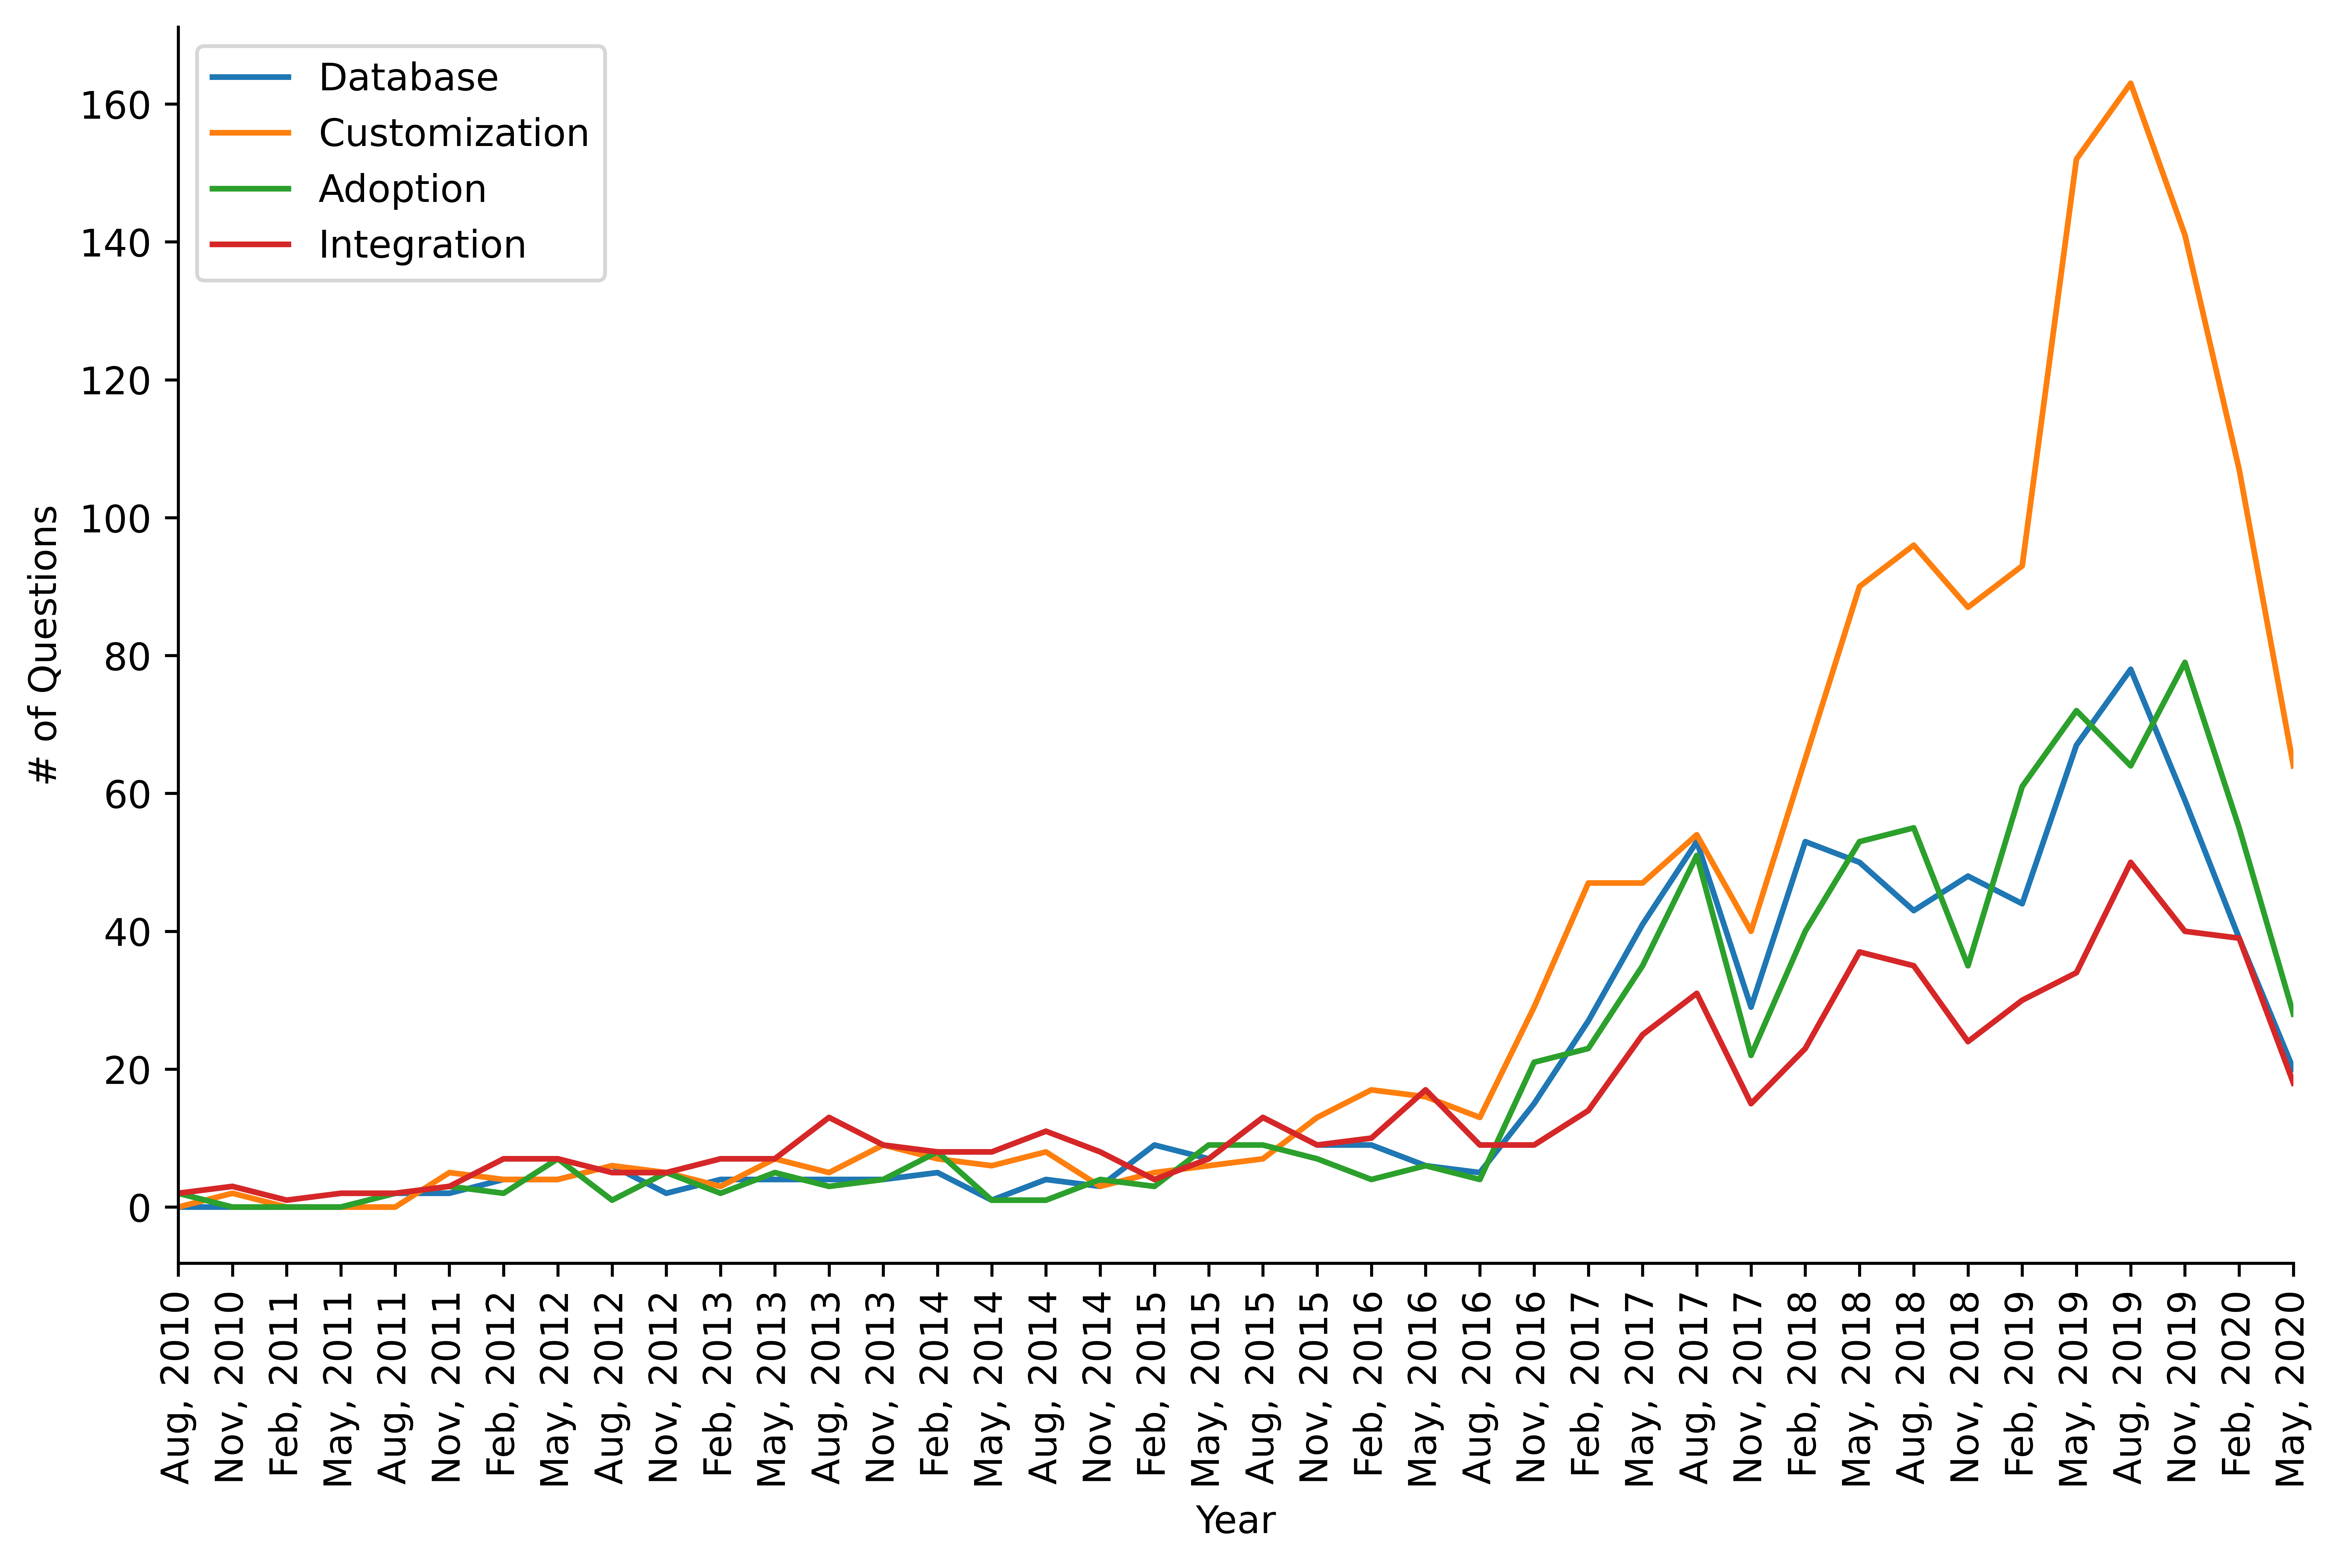
\includegraphics[scale=0.38]{res/Question_per_higher_category.png}
% 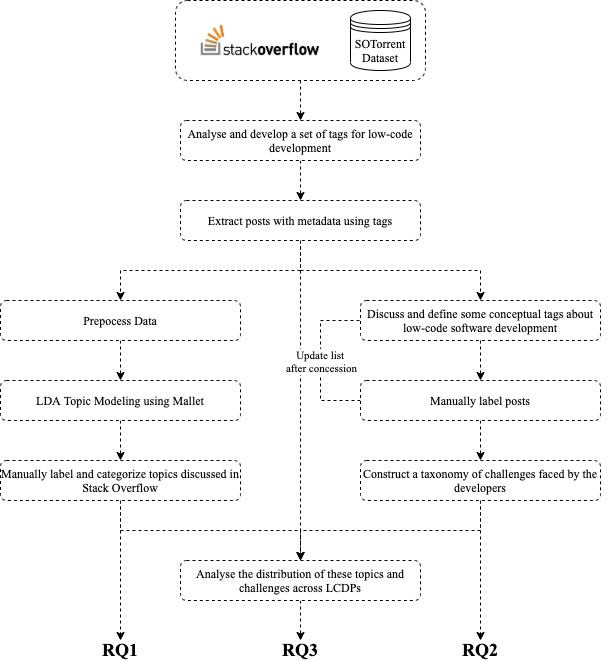
\includegraphics[width=0.35 * linewidth]{res/methology_overview.jpg}
\caption{Low-code topic category evolution over time.}
\label{fig:trend_questions_per_topic_category}
\end{figure}

\begin{figure}[t]
\centering
% 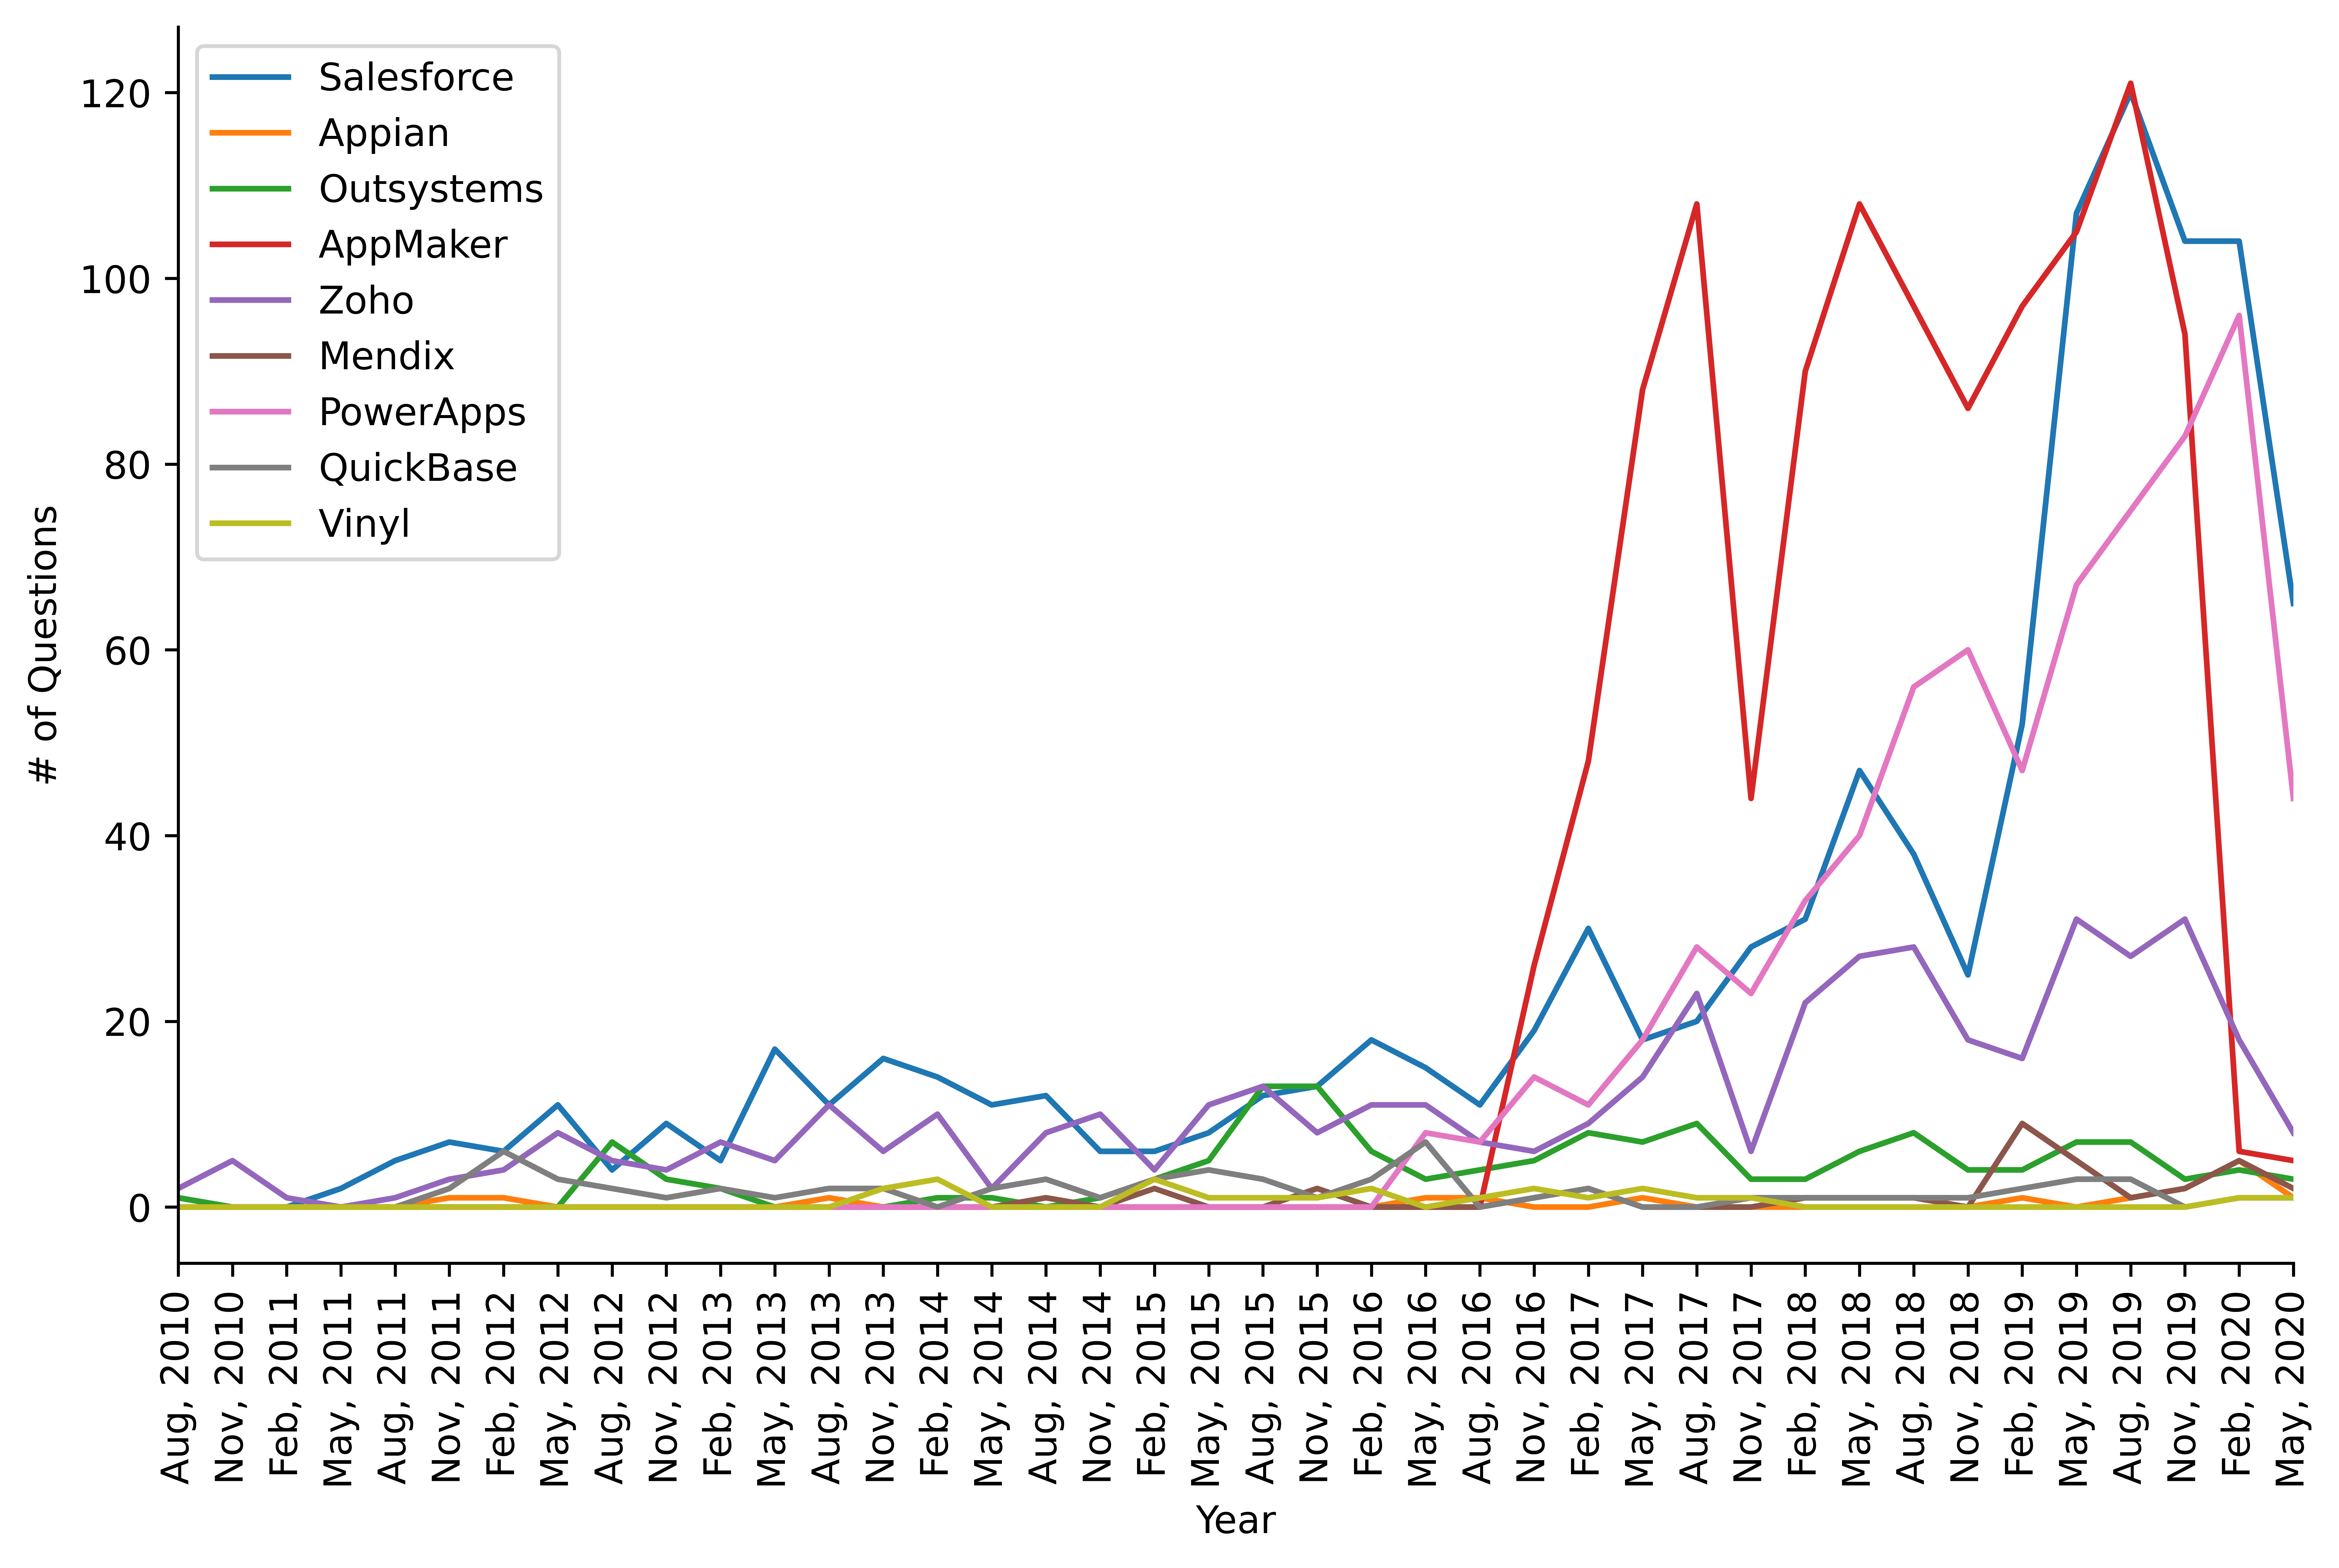
\includegraphics[scale=0.38]{res/question_per_platform.png}
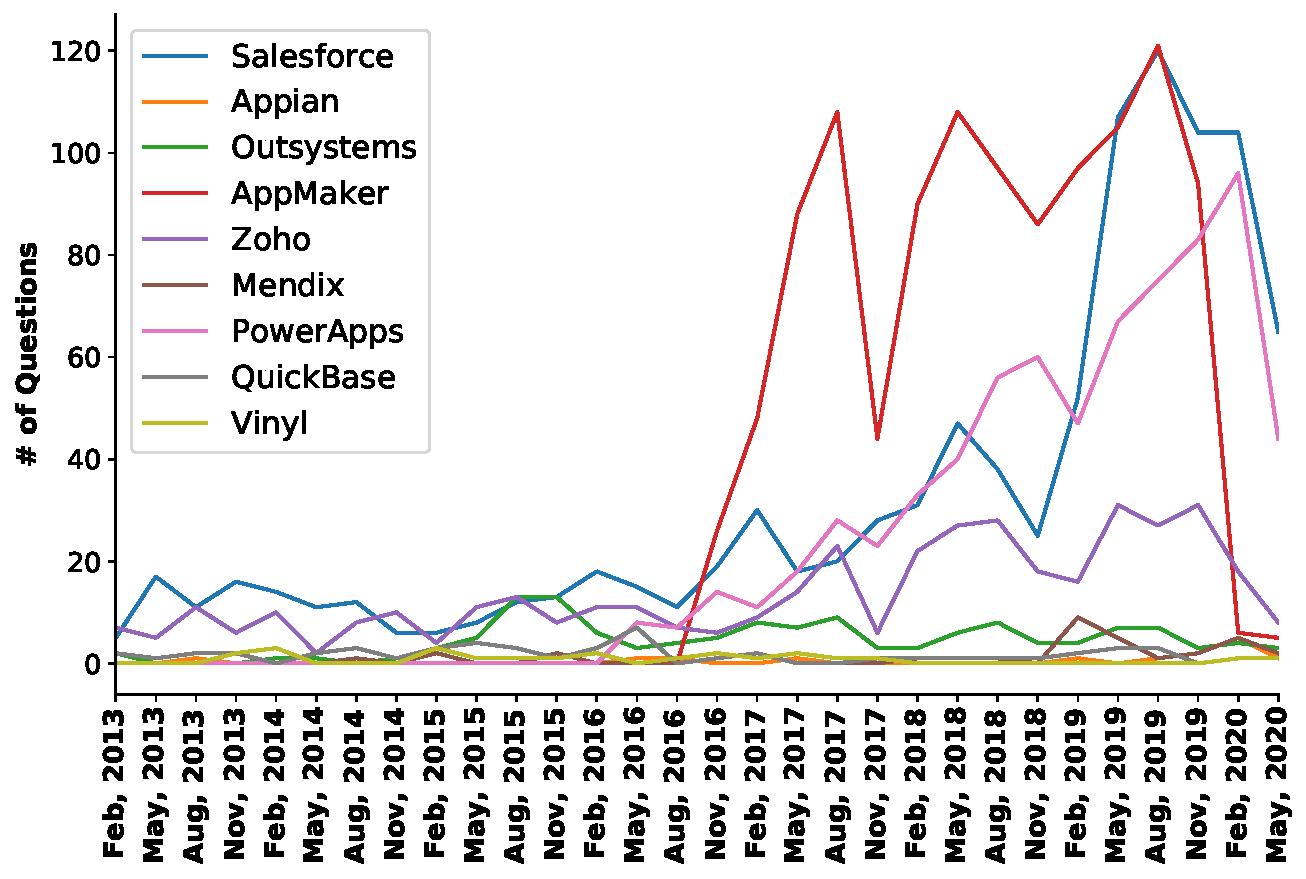
\includegraphics[scale=0.38]{res/question_per_platform_3M.pdf}
\caption{Low-code Platforms evolution over time}
\label{fig:trend_questions_per_platform}
\end{figure}

We further analyze two sudden swings in the number of questions. First, we find an increase of questions in every category after mid-2016, especially for questions about the \textit{Customization} category. Google released App Maker~\cite{googleappmaker} for public use in 2016, which introduced many discussions on LCSD customization. \fig\ref{fig:trend_questions_per_platform}  confirms it and shows a spike in questions about Google App Maker during that time. The second case is that at the beginning of 2020, there is a sharp decline in SO discussions. In Jan 2020, Google announced that they would no longer release new features for Google App Maker and discontinue it by 2021~\cite{google-disc}. It created unrest among the developer community as they were trying to verify this information (\dq{59947680}) and to explore alternatives (e.g., \dq{59985750}). \fig\ref{fig:trend_questions_per_platform} also shows the sudden drop in the number of questions asked about Google App Maker starting Jan 2020.
%Apart from this incident, there has been an overall increasing trend of  LCSD related discussions in SO despite the effect of Global pandemic during the early 2020.

%We also make our dataset publicly available \cite{}. \anindya{It would be an anonymous Git repo link in the footnote, not a citation.} 
%In summary,  LCSD is gaining community attention over time and
%our finding suggests that low-code community tends to pick up new LCSD platforms
%quite positively.


\subsection{Implications of Findings} 

% \gias{Here we will create two charts: (1) A bubble chart like Fig. 4 of Bagerzadeh and Khatchadourian~\cite{Bagherzadeh-BigdataTopic-FSE2019} and (2) the evolution of each challenge type over time by plotting the total number of times each challenge type is found per month. We will use the two charts to discuss the implications of findings}
% % follow Section 4 of \cite{Bagherzadeh-BigdataTopic-FSE2019}

\begin{figure}[t]
%\centering
\vspace{-5mm}
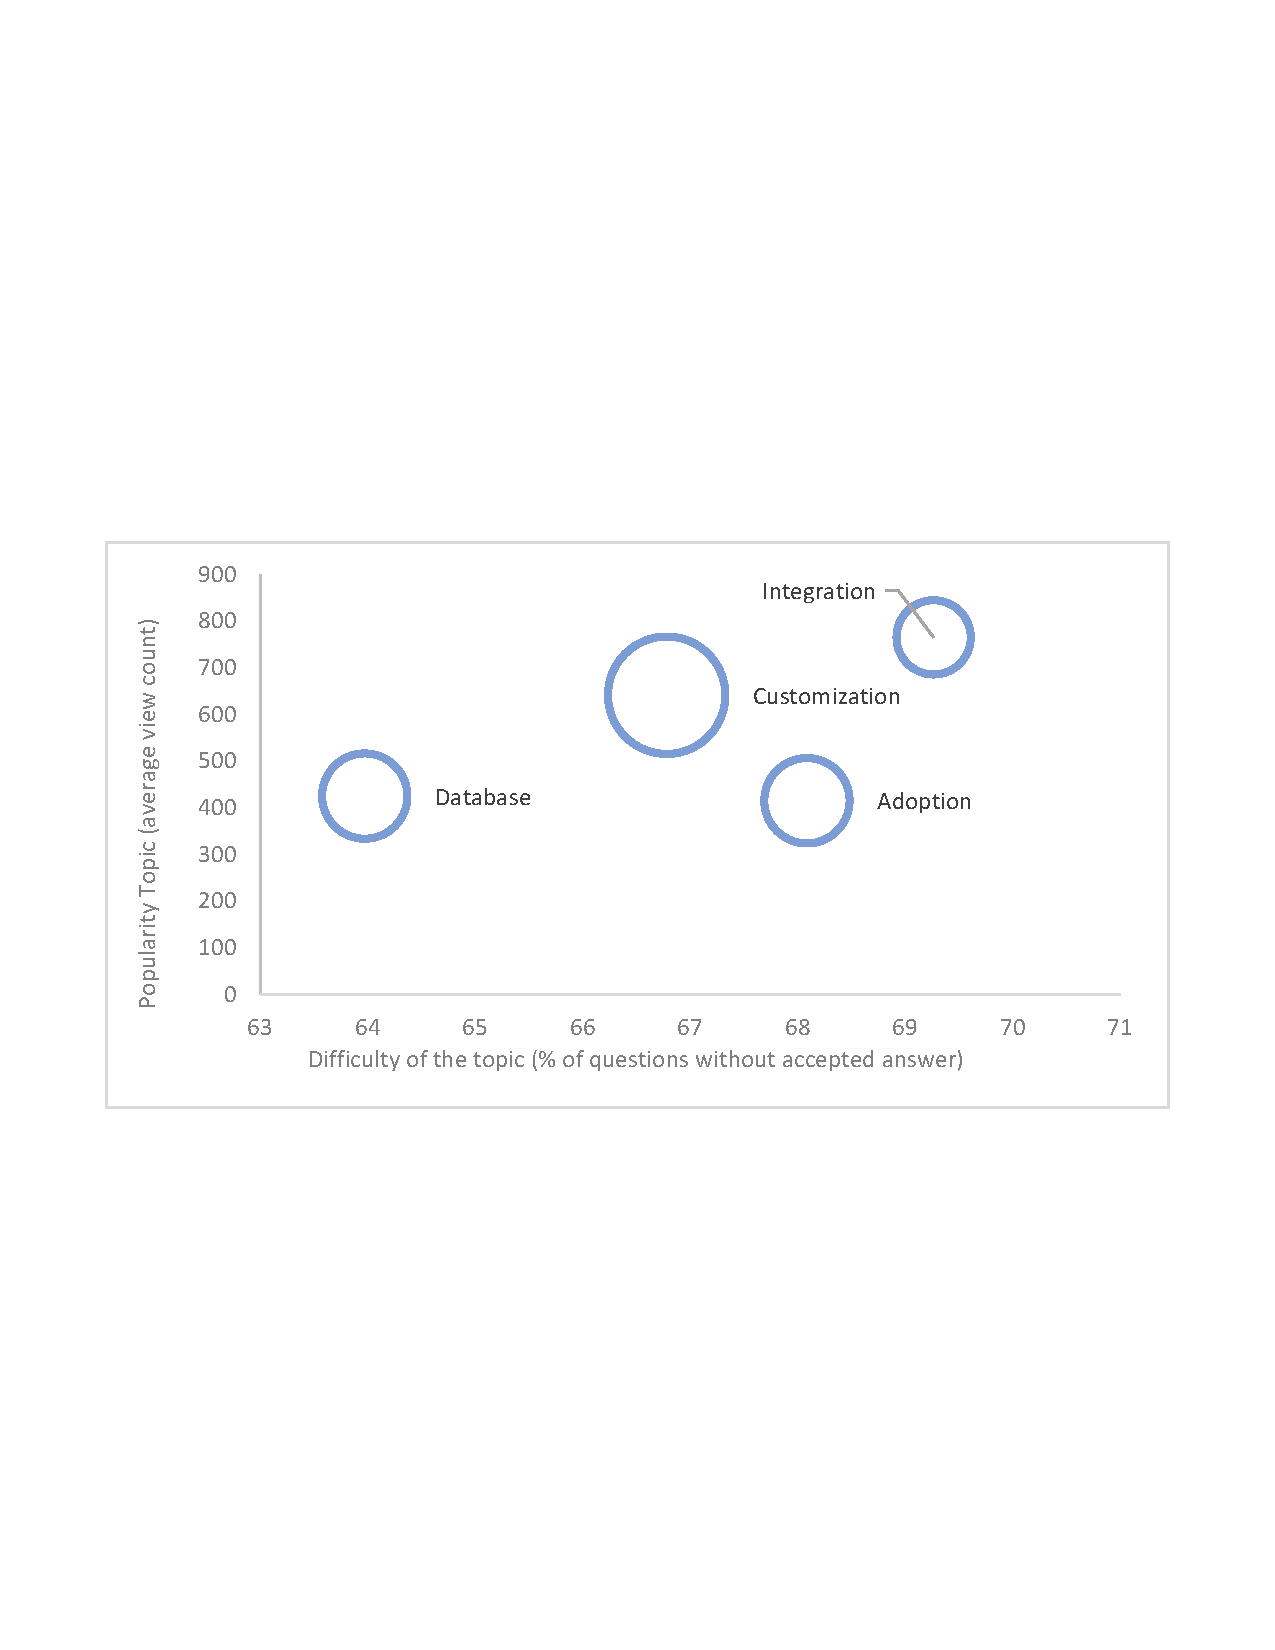
\includegraphics[scale=0.36]{res/popularity_difficulty_bubble_chart.pdf}
\vspace{-15mm}
\caption{Low-code topic categories popularity vs. difficulty}
\label{fig:bubble_diff_pop_per_category}
%\vspace{-5mm}
\end{figure}


% \begin{figure}[t]
% \centering
% 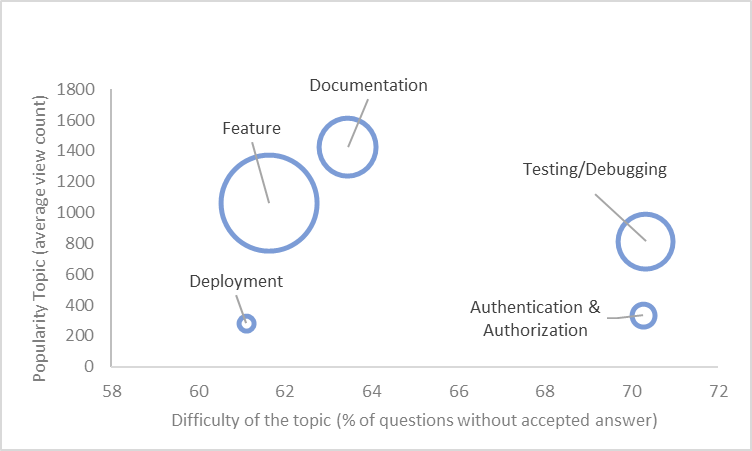
\includegraphics[scale=0.65]{res/bubble_diff_pop_per_challenge.png}
% % 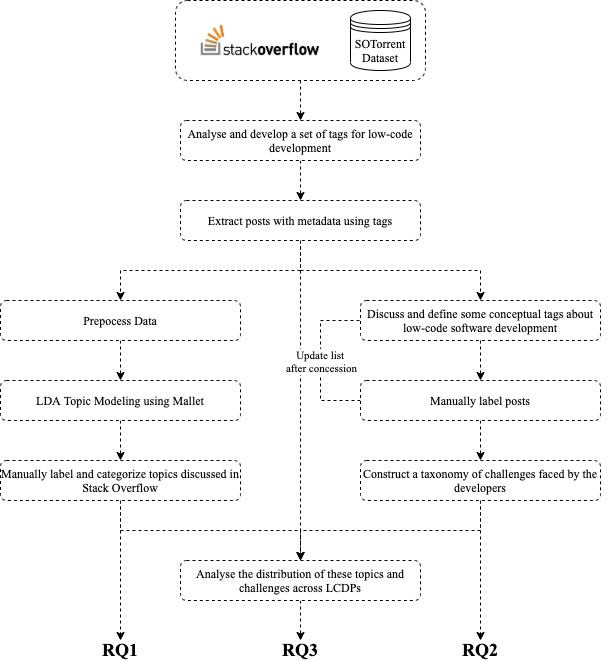
\includegraphics[width=0.35 * linewidth]{res/methology_overview.jpg}
% \caption{Low-code development challenges' popularity vs difficulty}
% \label{fig:bubble_diff_pop_per_challenge}
% \end{figure}

This study can help the low-code community to focus on the pressing issues on the
LCSD paradigm. We discuss the implications of our study findings by stakeholders below.

\bf{\ul{ LCSD Platform Providers.}} 
In order to better understand the issues of LCSD, we present a bubble chart \ref{fig:bubble_diff_pop_per_category} that presents the positions
of low-code categories in terms of popularity vs. difficulty. In this study, we
use the average number of view-count and percentage of questions without accepted
answers as a proxy for the topic category popularity and difficulty,
respectively~\cite{abdellatif2020challenges}. The size of the bubble depends on
the number of questions for that particular topic category.
Figure \ref{fig:bubble_diff_pop_per_category} shows that \textit{Integration} is
the most popular as well as most difficult topic category. On the other hand,
\textit{Database} remains the least difficult category due to the superior database support by  LCSD platforms. As shown in Figure \ref{fig:bubble_diff_pop_per_category},
\textit{Customization} is the largest and prevalent low-code topic category.
Many new practitioners make queries regarding LCSD platforms,
learning resources, basic application and UI customization, and how to get
started with this new emerging technology. We find that \textit{Documentation}
related queries are both very popular and difficult. Our
findings also suggest that many practitioners still face challenges during testing and debugging. Consequently, many of
the questions on this topic remain unanswered. It reveals that to ensure smooth adoption of the LCSD platform, the platform providers should provide better and effective documentation and provide learning resources to reduce entry-level barriers and smooth out the learning curve. 

\textbf{\ul{ LCSD Practitioners/Developers.}} LCSD abstractions and the platform's
feature limitations sometimes make it very difficult to customize and debug. Our
finding shows that the practitioners find third party service \textit{Integration}
and \textit{Platform Feature} category most difficult. It provides valuable
insights for project managers to manage resources better (i.e., human resources and
development time). 
% \anindya{example of integration issue?} 
LCSD platform enables practitioners with diverse experience to contribute to the development process even without a software development
background. However, our finding shows that practitioners find debugging, application
accessibility, and documentation challenging. Hence, the practitioners should take
the necessary steps to understand the tradeoffs LCSD platforms' features deeply. The project manager should adopt specific strategies to learn to customize, debug, and test the application.


\textbf{\ul{ LCSD Researchers \& Educators.}} We find that
the LCSD paradigm's challenges can be different from traditional software development~\cite{sahay2020supporting}. Researchers can focus on the most popular
and difficult topic category \textit{Integration} and
develop a set of metrics to automatically detect documentation quality on
third-party service APIs. Simultaneously, researchers can study how to
provide better tools for practitioners to customize the application.
Security is an open research opportunity for such platforms as a security
vulnerability in such platforms or frameworks could compromise millions of applications and users~\cite{lin2020software}. Researchers can come
up with better testing approaches to ensure faster development and dependability. Educators can also benefit from the results presented in Figure
\ref{fig:bubble_diff_pop_per_category} to prioritize their focus on different topics such as \textit{Database, Customization, and Third-party API Integration}.

% There are many factors that can contribute to the LCSD adoption. Low-code
% researchers, practitioners, platform providers need to consider these factors
% and their trade offs. However, we believe our findings and implications can help
% the decision making process.

% Low-code development platforms has a still long way to go. Practitioners still face difficulty to design UI and application customization and data store. There are lots of research opportunity to improve security, better automatic code generation, server deployment.



% lack of security and scalability discussion

% \paragraph{Community support}
% \paragraph{Community support}
% \paragraph{Documentation/Tutorial support}
% \paragraph{Future software development}

% \paragraph{Training}

% \subsection{Threats to Validity} \label{subsec:validity}
% There are some threats that may affect the validity of our study results. 
% \paragraph{Internal Validity}
% The internal threat refers to the mistakes or errors in our experiments such as missing some related questions regarding low-code development if the questions have not been tagged properly. We double checked to find related tags. There might be some making coding error during LDA topic modelling and SO post extractions. This data extraction have have reviewed by two authors. Our studied X SO posts regarding LCDP. We selected these posts by choosing questions that has at least one tags of some popular LCDP. We have not takes posts that does not have LCDP tags. we reported LDA parameters for replications
% 
% Tags were selected in an open debate session
% difficult to find optimal value of K. We used different values of K and calculated topic coherence score. As LDA is probabilic, we ran our model couple of times and find not significant difference.
% 
% We tried several well known techniques to extract related tags \cite{rosen2016mobile}\cite{bagherzadeh2019going}.
% We tried several well known techniques to manual labelling \cite{bajaj2014mining}\cite{ahmed2018concurrency}.
% We tried several well known techniques to find k \cite{ahmed2018concurrency}\cite{barua2014developers}.
% 
% 
% Only SO might not show the whole picture because due the platform's question's policies, there are some non technical but important challenges such as general soft ware architecture/design questions, comparison between platforms, platform's reputation, support and scalability,
% However large number of  SO questions and community members comments help to mitigate this.
% 
% 
% 
% 
% 
% \paragraph{External Validity}
% 
% Our work does not cover entire low-code ecosystem..
% The external threat to our study can be the generalization that we provided on the challenges that the developers have at different stages of low-code software life cycle. Manual labelling of questions is generally biased but we tried to reduce it taking votes of 4 Authors when there is conflict. After discussion we had around ? percent agreement.
% We have conducted this study by study around ? SO questions and manually reviewing ? questions by four authors. In the future we intend to address this issue by interviewing low-code developers and getting their feedback on our generalization, analysing data from different sources. 
% 
% Further studies should include more data sources.




% \begin{figure}[t]
% \centering
% \hbox{\hspace{-3em}\includegraphics[scale=0.42]{res/questions_per_platform_Per_Two_Month_With_Total.png}}
% % 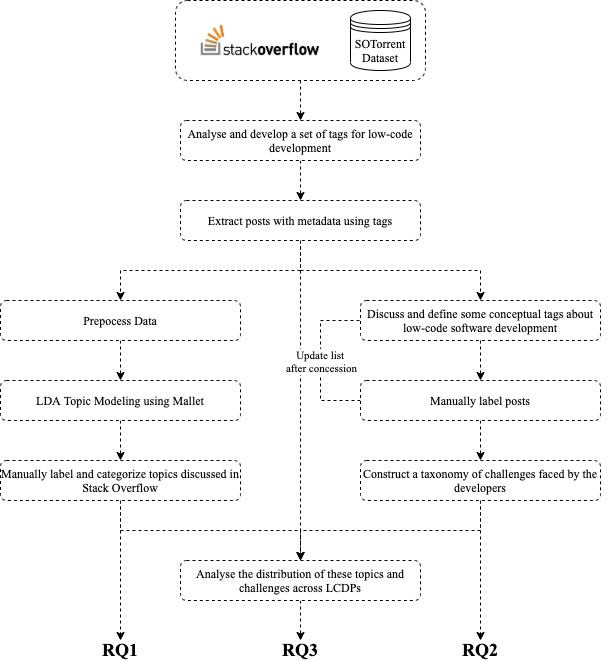
\includegraphics[width=0.35 * linewidth]{res/methology_overview.jpg}
% \caption{Trend of discussions on SO on different low-code development platforms over time}
% \label{fig:questions_trend_per_lcdp_platform}
% \end{figure}
% 
% \begin{table}[htb]
%     \caption{Low-code software development platforms, their popularity, and their significance }
%     \centering
%         \begin{tabular}{|m{5em}|m{10em}|m{2em}|m{3em}|m{3.5em}|}%         
%         \hline
%         \textbf{Platform Name} & \textbf{Tag Name} & \textbf{\# of Posts} & \textbf{Avg view count} & \textbf{Avg favorite count}\\%         
%         \hline
%         \textbf{Salesforce} & salesforce-lightning \newline lwc \newline lightning \newline salesforce-communities \newline salesforce-chatter \newline salesforce-service-cloud \newline aura-framework & 1031 & 619.75	
%  & 1.05 \\%     
%         \hline
%         \textbf{Appian} & appian & 16 &	366.56 &	2  \\%         
%         \hline
%         \textbf{OutSystems} & appian & 147 & 1156.93 & 1.31  \\% 
%         \hline
%         \textbf{AppMaker} & google-app-maker & 1123 & 272.36 & 1.07 \\%         
%         \hline
%         \textbf{Zoho} & appian & 445 & 874.95	& 1.26 \\% 
%         \hline
%         \textbf{Mendix} & mendix & 35 &	459.74 &	1  \\%   
%         \hline
%         \textbf{PowerApps} & powerapps \newline powerapps-formula \newline powerapps-selected-items \newline powerapps-collection \newline powerapps-canvas & 710 &	684.54 & 1  \\% 
%         \hline
%         \textbf{QuickBase} & quickbase & 67 & 575.02 &	0.9  \\% 
%         \hline
%         \textbf{Vinyl} & vinyl & 23	& 289.39	& 1  \\% 
%         \hline
%         \end{tabular}
%     
%     \label{tab:LCDPs_questions_distribution}
% \end{table}
% 
% 
% 
% 
% \begin{figure}[htb]
% \centering
% 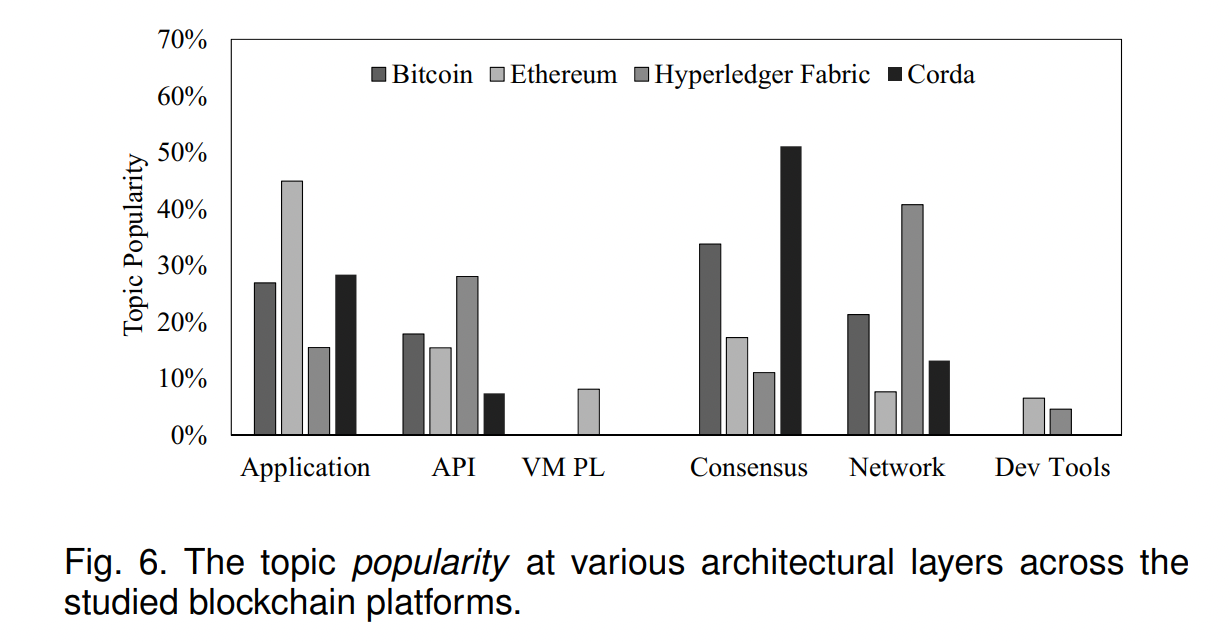
\includegraphics[scale=0.40]{res/bar_block_chain.png}
% % 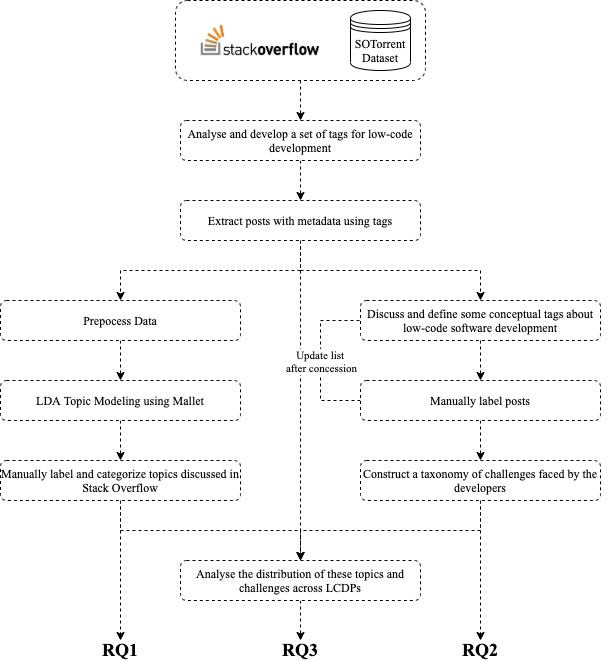
\includegraphics[width=0.35 * linewidth]{res/methology_overview.jpg}
% \caption{(Dummy) How practitioners face challenges in different stages of agile development life cycle in different low-code development platforms over time.}
% \label{fig:challenges_per_lcdp}
% \end{figure}
% 
% \begin{figure}[htb]
% \centering
% 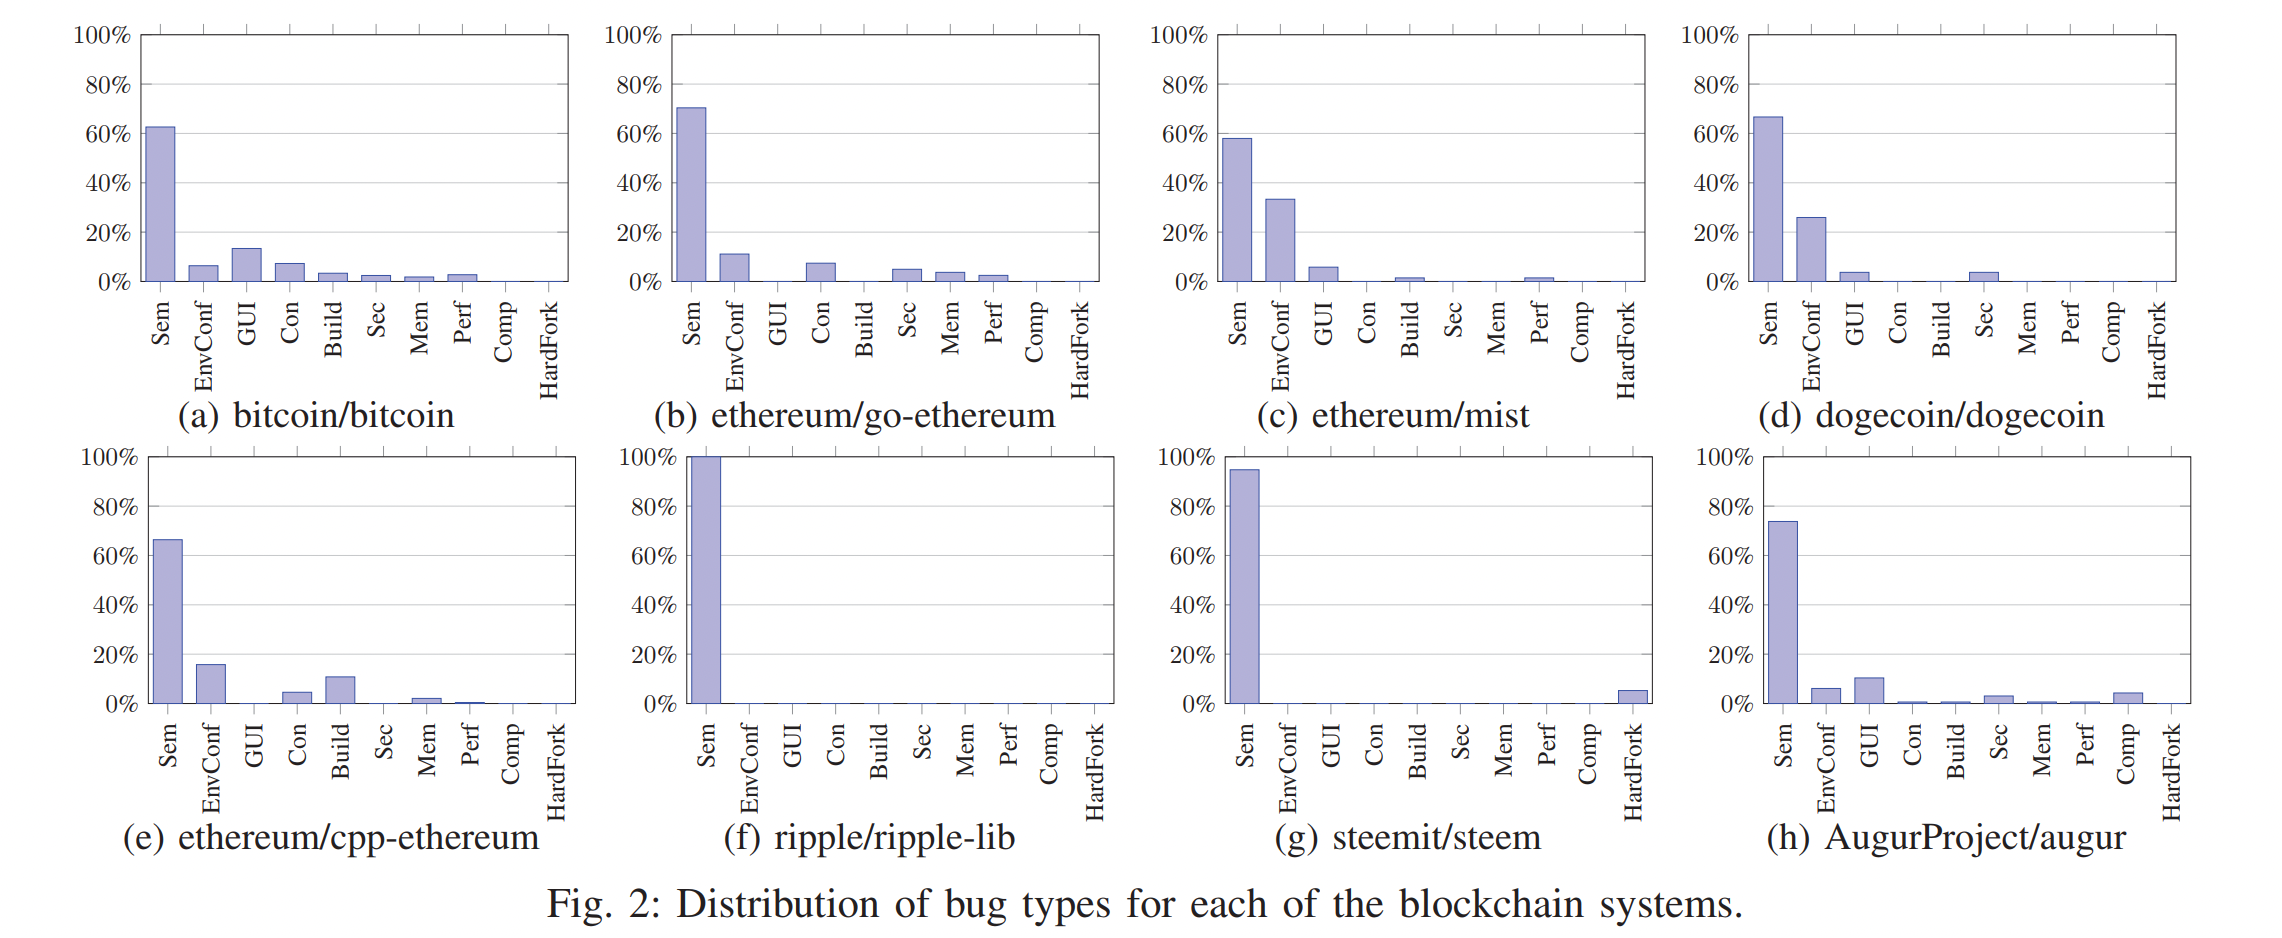
\includegraphics[scale=0.22]{res/bug_accross_platform.png}
% % 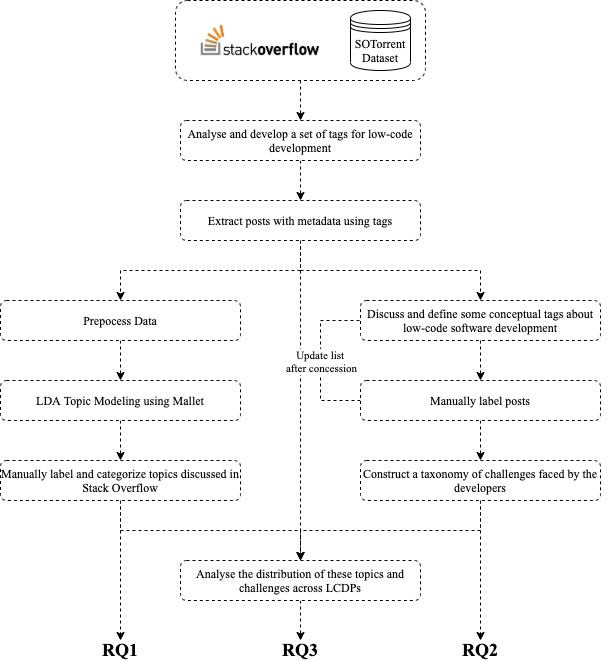
\includegraphics[width=0.35 * linewidth]{res/methology_overview.jpg}
% \caption{(Dummy) How topics are distributed across different low-code development platforms over time.}
% \label{fig:topics_per_lcdp}
% \end{figure}
% 
% 
% 
% 
% \subsubsection{Motivation} 
% % motivate why this research question is important
% Different LCDPs have different set of features, advantages and disadvantages. 
% % For example, Salesforce ? this ? is easier. ? platform provides ? 
% In this research question, we discuss on discussions related to different challenging topics distribute across different low-code development platforms. This will provide valuable insights of about different LCDPs and their usability cases.
% 
% \subsubsection{Approach} 
% % categorize each question+accepted answer by the low code provider tagged or discussed (e.g., zoho, appian, etc.).
% We started with top 9 low-code development platforms (Salesforce, Appian, OutSystems, App Maker, Zoho, Mendix, PowerApps, QuickBase, Vinyl) as presented in Table \ref{tab:LCDPs_questions_distribution}. From our RQ1, we found posts categorized in 5 higher level of topics and from RQ2, we manually labelled ? posts into different technological challenges faced during development. For this research questions we find out how these technical topics and challenges are distributed across different LCDPs.
% 
% % From our manual labeling of questions, and our taxonomy presented \ref{} we showed
% 
% \subsubsection{Results} 
% % report the results
% 
% Table \ref{tab:LCDPs_questions_distribution} shows how many questions are asked about different LCDPs, and popularity and impact. We can see that, in SO the Salesforce(1031) and AppMaker (1157) are the most discussed LCDP and each has more than one thousands of posts. Zoho and PowerApps are second most popular LCDPs, they have around half thousand posts each. Appian, OutSystems, Mendix, QuickBase, Vinyl have around one hundred posts each. Posts in OutSystems have the highest average view count (1157) and Google app maker has the lowest average view count (272). Figure \ref{fig:questions_trend_per_lcdp_platform}  
% and it also shows that total number of discussions on low-code development is increasing over and it also how discussions across different low-code platform are evolving over time.
% 
% Figure \ref{fig:topics_per_lcdp} shows how various topics derived from our topic modeling are distributed across LCDPs. We can see that topic ?, ? and ? is more prevalent in platform ?. Platform ? has the highest number of discussion on ?, ?. ? is also more discussed in platform ?.
% 
% Figure \ref{fig:challenges_per_lcdp} show how different type of challenges are more prevalent across different LCDPs.  We can see ?, ? have more discussion on ?. Discussion related to debugging is more prevalent in ?. In ? there are a lot of posts regarding cloud configuration. ? has quite a few discussion on UI and Application customization. ? has a lot of queries on deployment and user role management.
